\begin{figure}[H]
  \centering
  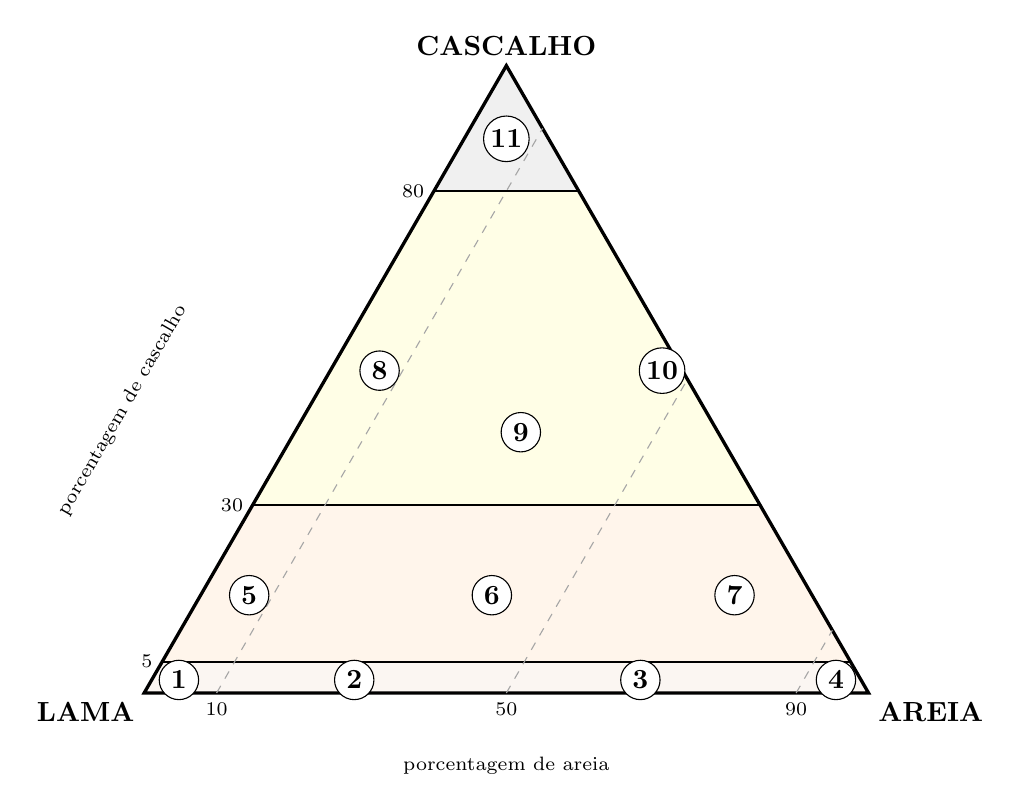
\begin{tikzpicture}[x=0.92cm,y=0.92cm,font=\scriptsize]
    \coordinate (M) at (0,0);
    \coordinate (S) at (10,0);
    \coordinate (G) at (5,8.66);

    % Campos granulométricos principais
    \path[fill=brown!7] (M)--(S)--(9.75,0.433)--(0.25,0.433)--cycle;
    \path[fill=orange!8] (0.25,0.433)--(9.75,0.433)--(8.5,2.598)--(1.5,2.598)--cycle;
    \path[fill=yellow!10] (1.5,2.598)--(8.5,2.598)--(6,6.928)--(4,6.928)--cycle;
    \path[fill=gray!12] (4,6.928)--(6,6.928)--(G)--cycle;

    % Contorno e limites de porcentagem de cascalho
    \draw[very thick] (M)--(S)--(G)--cycle;
    \draw[thick] (0.25,0.433)--(9.75,0.433); % 5% cascalho
    \draw[thick] (1.5,2.598)--(8.5,2.598);   % 30% cascalho
    \draw[thick] (4,6.928)--(6,6.928);       % 80% cascalho

    % Limites de porcentagem de areia
    \draw[gray!70,dashed] (1,0)--(5.5,7.794);   % 10% areia
    \draw[gray!70,dashed] (5,0)--(7.5,4.330);   % 50% areia
    \draw[gray!70,dashed] (9,0)--(9.5,0.866);   % 90% areia

    % Polos e eixos
    \node[above,font=\bfseries] at (G) {CASCALHO};
    \node[below left,font=\bfseries] at (M) {LAMA};
    \node[below right,font=\bfseries] at (S) {AREIA};
    \node[rotate=60] at (-0.30,3.9) {porcentagem de cascalho};
    \node[below] at (5,-0.75) {porcentagem de areia};
    \node[left] at (0.25,0.433) {5};
    \node[left] at (1.5,2.598) {30};
    \node[left] at (4,6.928) {80};
    \node[below] at (1,0) {10};
    \node[below] at (5,0) {50};
    \node[below] at (9,0) {90};

    % Numeração dos campos; a nomenclatura aparece na lista abaixo.
    \tikzset{campo/.style={circle,draw,fill=white,inner sep=1.2pt,
      minimum size=5mm,font=\bfseries}}
    \node[campo] at (0.48,0.18) {1};
    \node[campo] at (2.90,0.18) {2};
    \node[campo] at (6.85,0.18) {3};
    \node[campo] at (9.55,0.18) {4};
    \node[campo] at (1.45,1.35) {5};
    \node[campo] at (4.80,1.35) {6};
    \node[campo] at (8.15,1.35) {7};
    \node[campo] at (3.25,4.45) {8};
    \node[campo] at (5.20,3.60) {9};
    \node[campo] at (7.15,4.45) {10};
    \node[campo] at (5,7.65) {11};
  \end{tikzpicture}

  \vspace{0.5em}
  \begin{tabularx}{0.98\linewidth}{@{}rX rX@{}}
    \toprule
    \multicolumn{4}{c}{\textbf{Nomenclatura dos campos}} \\
    \midrule
    1. & Lama / pelito
       & 7. & Areia cascalhosa / arenito cascalhoso \\
    2. & Lama arenosa / pelito arenoso
       & 8. & Cascalho lamoso / conglomerado lamoso \\
    3. & Areia lamosa / arenito lamoso
       & 9. & Cascalho areno-lamoso / conglomerado areno-lamoso \\
    4. & Areia / arenito
       & 10. & Cascalho arenoso / conglomerado arenoso \\
    5. & Lama cascalhosa / pelito cascalhoso
       & 11. & Cascalho / conglomerado \\
    6. & Areia lamosa cascalhosa / arenito lamoso cascalhoso
       & & \\
    \bottomrule
  \end{tabularx}
  \caption{Classificação textural de sedimentos e rochas formados por misturas de
  cascalho, areia e lama. Os limites de 5, 30 e 80\% referem-se à proporção de
  cascalho.}
  \label{fig:classificacao-conglomerados}
  \caption*{\footnotesize Fonte: adaptado de \textcite{nichols2009}.}
\end{figure}
